\documentclass[../thesis/thesis.tex]{subfiles}
\renewcommand{\baselinestretch}{1.5}\selectfont
\graphicspath{{../figs/ch1-intro/}}

\begin{document}
\begin{refsection}
\chapter{Introduction}
\section{Motivation}

Telecommunications underpins our modern world. Both business and leisure in developed nations rely on the connectivity of digital devices, and around the world mobile telecoms provides critical services in emergencies. The use of mobile devices continues to rise year-on-year at a rate such that it is predicted there will be 8.4 billion mobile broadband internet subscriptions by 2024 \cite{Ericsson_2019}, as shown in Figure \ref{ch1_fig_ericsson}. To achieve the bandwidth and latency requirements for this increasing number of users, new technologies are in continuous development. The next iteration to be deployed, the fifth-generation cellular network technology (5G), uses substantial hardware innovations to satisfy these requirements. One of the most significant changes in 5G networks is a dramatic increase in the number of base stations required to serve mobile devices. This is a cause for concern due to the energy efficiency of the high power amplifiers in the final stage of the base station, which amplify the output of the network systems to drive the wireless antennas. In addition, the efficiency of the smaller amplifiers in mobile devices is important due to the billions of them in use.

\begin{figure}
	\centering
	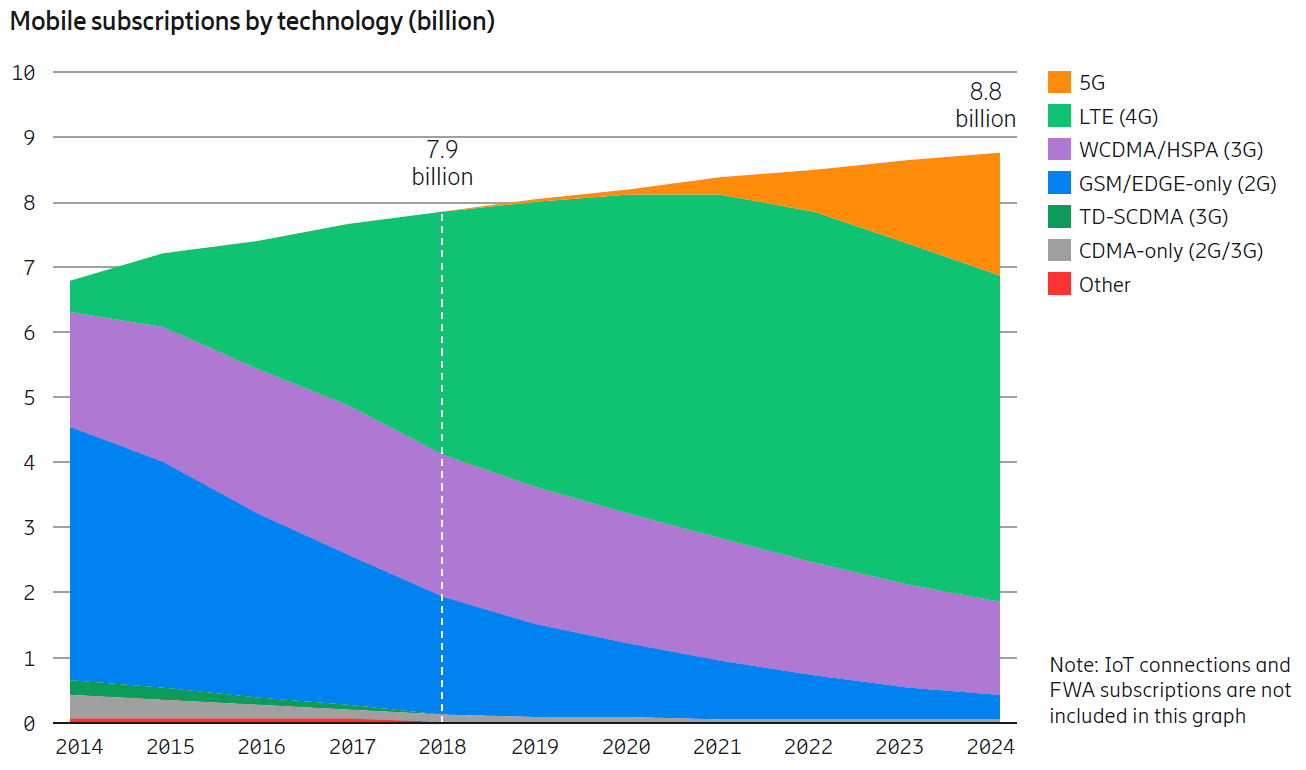
\includegraphics[width=\textwidth]{ch1_ericsson}
	\caption{The past and predicted future trends of global mobile subscribers \cite{Ericsson_2019}.}
	\label{ch1_fig_ericsson}
\end{figure}

We are increasingly aware of the effects of climate change and our responsibility to reduce our impact on the environment in which we live. Energy consumption is a key area where this can be addressed, so it is desirable to improve the efficiency of new cellular amplifiers, especially if many more will soon be deployed. From a communications perspective, the ideal choice is a linear amplifier, however the efficiency of such amplifiers is limited to 50\% \cite{Cripps_2006}. Alternatively, amplifiers operated in the nonlinear regime can use methods which are not fundamentally limited in their efficiency, with recent performance as high as 70\% \cite{Kosaka_2016,Bhardwaj_2019}. The problem with using nonlinear amplifiers for communications is that they distort the signal, causing errors in the received data unless this distortion is corrected for. Fortunately, this correction is available as digital pre-distortion (DPD). To design a nonlinear amplifier using DPD, engineers rely on accurate models of the active device (a radio-frequency (RF) power transistor), an example of which is shown in Figure \ref{ch1_fig_rfpa}. These models are a critical part of the amplifier design process and many large-scale manufacturers have a dedicated team of engineers devoted to developing them. There are three main categories of model in use \cite{Aaen_2007}:

\begin{itemize}
	\item \emph{Physical models} are defined by the fundamental equations which govern the internal structure and materials of the transistor. They are used in the early stages of the design process when the transistor die itself is developed. Due to their computational complexity they are not used in later packaged amplifier or system simulation stages.
	\item \emph{Compact models} represent the packaged transistor, which contains the transistor die, any required matching components and parasitic package effects. They are either defined as equivalent-circuit parameters or a simplified set of physical relationships which are applicable at the packaged device terminals. The coefficients of the model are found during extraction, where various measurements are made of the device and the model is fitted to the results. Compact models can be used in circuit simulators to integrate transistors into full amplifier systems, which can contain multiple transistors and passive components.
	\item \emph{Behavioural models} are entirely measurement based and their form is not dependent on the internal structure of the device. This ``black-box'' approach is very attractive to industry as it minimises the intellectual property which must be shared with users of their product. In addition, less time is spent when compared to validating a custom compact model. Like compact models, behavioural models are used in circuit simulators at the amplifier design stage.
\end{itemize}

\begin{figure}
	\centering
	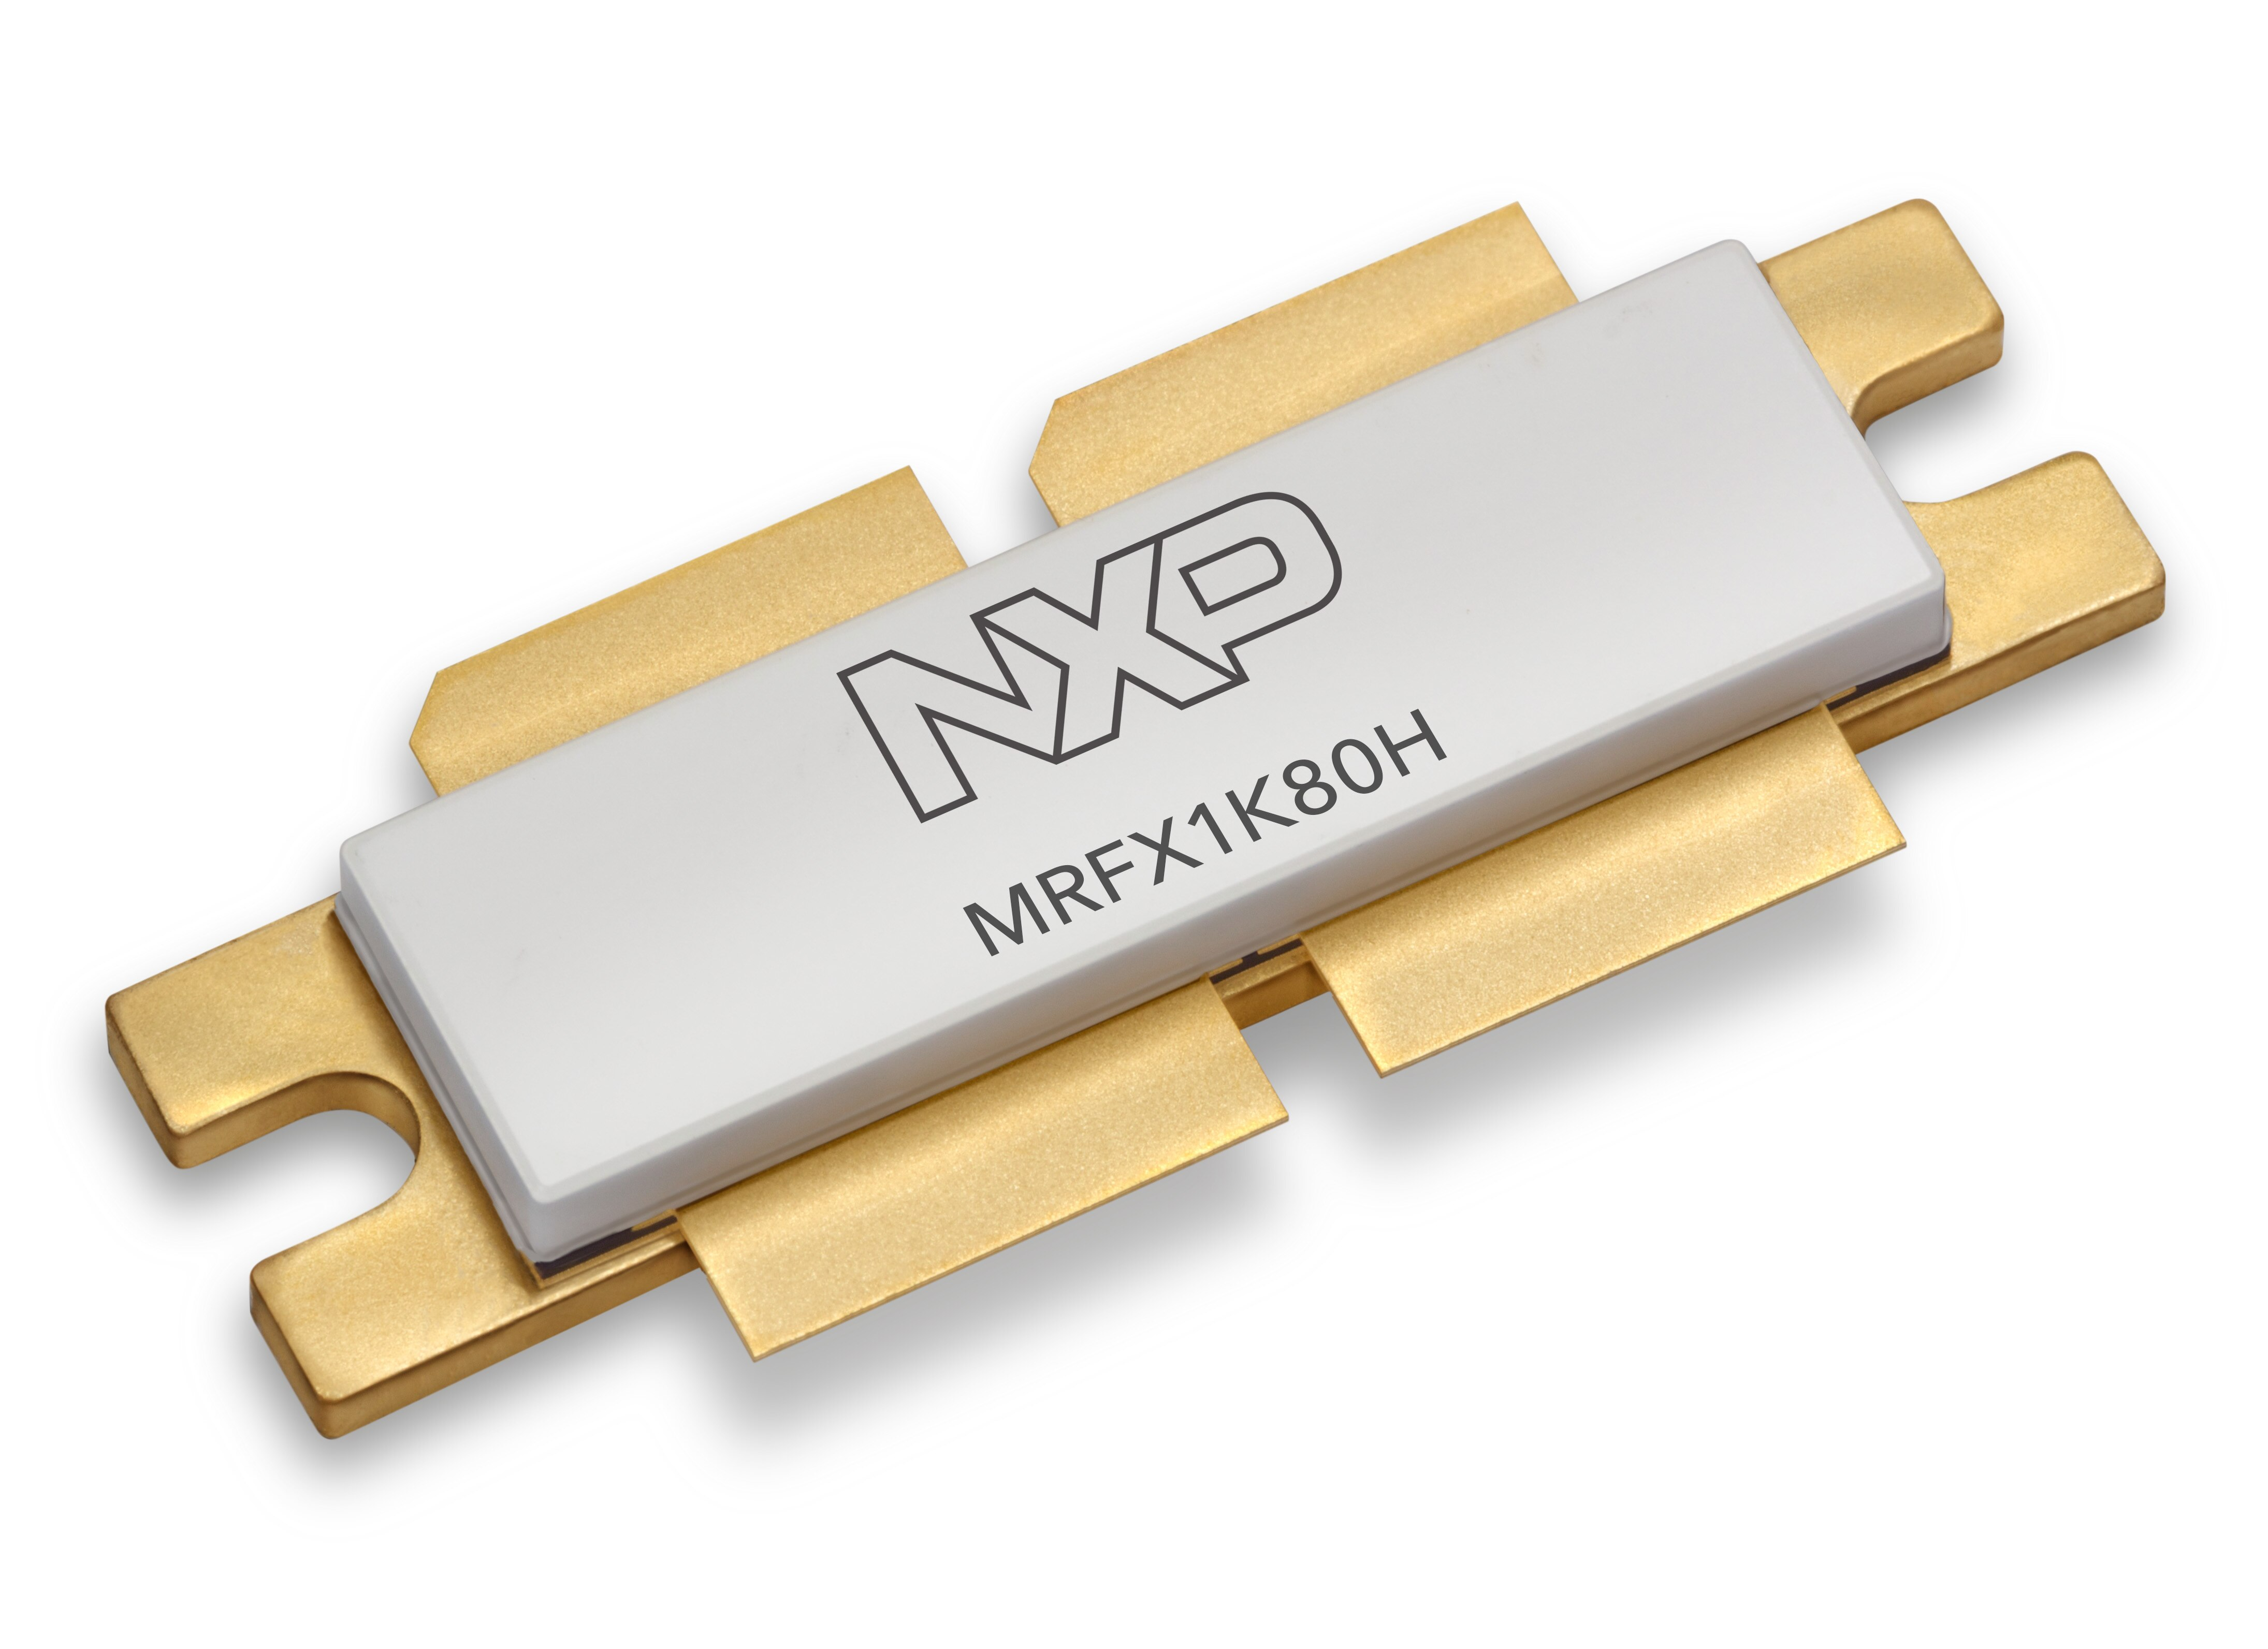
\includegraphics[width=0.6\textwidth]{ch1_rfpa}
	\caption{A typical packaged RF power transistor \cite{blf861a}.}
	\label{ch1_fig_rfpa}
\end{figure}

Between the foundry, transistor manufacturer and amplifier designer, all three categories of model may be used for a particular product. It is important in this competitive industry for fast time-to-market and therefore first-pass design success is a popular target for amplifier designers. To enable this, transistor models must be as accurate as possible to ensure the simulated performance matches the physical reality. Measurements of transistors are critical to both compact and behavioural models, which means the quality and confidence of those measurements are a significant factor in increasing device performance.

To provide confidence in measurements, an evaluation of any uncertainty in their result is required. All measurements have sources of error which contribute to uncertainty, and the science of metrology is concerned with quantifying and minimising these uncertainties in measurement. Due to the prevalence of measurement in science and commerce, National Metrology Institutes (NMIs) exist, such as the National Physical Laboratory (NPL) in the UK, to improve confidence in measurements via traceability to National standards and the development of new techniques. The NMIs have included RF and microwave measurements in their role for many years, but the recent challenges from new cellular technologies presents further opportunity for new metrology. This includes increasing the upper frequency of linear device measurements to millimetre-wave and beyond for 5G network backbone applications, and incorporating measurement uncertainty into compact and behavioural models of nonlinear amplifiers. The latter point has significant benefits to the amplifier design community. Firstly, confidence in the extraction of the model can be quantified. This allows the designer to decide if the model is suitable and if first-pass design success is likely when compared with their tolerances and requirements \cite{Williams_2016B}. If the sensitivities to different sources of error are propagated into the model, then it is possible to make informed investments to improve the accuracy of relevant measurement instrumentation. Secondly, both compact and behavioural models do not recreate the device response perfectly, typically ignoring some higher-order effects. If measurement uncertainty from the model extraction is propagated into the model itself, then any remaining error between the model and the device measurements must be attributed to model inaccuracies \cite{Cheron_2018}. The research in this dissertation updates traditional NMI metrology for 5G and beyond, and introduces a method to incorporate measurement uncertainty into behavioural models of power amplifiers for use with 5G.

\section{Prior Research}

To understand the objectives of this dissertation, it is sensible to first summarise the prior research in this area.

Vector Network Analyser (VNA) metrology has been prevalent at NMIs for decades, resulting in the publication of guidance documents for laboratory use \cite{EA_2000,EURAMET_2011}. However, rigorous evaluations of VNA measurement uncertainty, which include all significant sources of error and propagates their uncertainties into the result, have only occurred relatively recently. These evaluations can support either of two different propagation techniques, or both. Numerical propagation, implemented using either Monte Carlo or finite-difference methods, only requires knowledge of the equations governing the measurement (the ``measurement model''). Analytical propagation is typically implemented using the Law of Propagation of Uncertainty (LPU) \cite{GUM_2008}, which requires the first-order derivatives of the measurement model to be derived. Although faster than numerical propagation, it cannot easily produce accurate probability distributions for the results of complicated measurement models which Monte Carlo methods can. For VNA measurements, rigorous uncertainty evaluations using numerical propagations has been demonstrated in \cite{Hoffman_2007}, and the popular software framework ``VNA Tools II'' from the Swiss NMI METAS provides a free easy-to-use implementation \cite{VNATools}. Analytical propagation is also provided by this software package using automatic differentiation techniques, and an explicit derivation can be found in \cite{Lewandowski_2010B}.

Nonlinear Vector Network Analysers (NVNAs) are used to perform the measurements required to extract compact and behavioural models of nonlinear amplifiers, and these instruments can be based on a modified version of a VNA. Recent research has built upon the knowledge of VNA metrology in order to adapt uncertainty evaluations to support NVNA measurements. Lin and Zhang provided the first uncertainty evaluation using analytical propagation in 2012 \cite{Lin_2012}, which has been followed by the Microwave Uncertainty Framework (MUF) software tool from the US NMI, NIST, providing numerical propagation methods \cite{MUFWebsite,Avolio_2015}.

The only propagation of measurement uncertainty into a nonlinear model of a microwave amplifier prior to the work covered in this dissertation was by Cheron et al. in 2018 \cite{Cheron_2018}. This evaluation of uncertainty used a numerical propagation provided by \cite{MUFWebsite} and extended the framework to include the extraction of parameters for a compact model. To date, there has been no published work regarding uncertainty evaluations for extracted behavioural models of nonlinear microwave amplifiers.

A concise view of prior research is shown in Table \ref{ch1_table_prior}. Further detail of the work summarised here is given in subsequent chapters.

\begin{table}[]
	\begin{tabular}{@{}lll@{}}
		\toprule
		Measurement        & Numerical Propagation & Analytical Propagation\\ \midrule
		VNA (S-parameters) & \cite{Hoffman_2007,VNATools}  & \cite{Lewandowski_2010B,VNATools}           \\
		NVNA (power waves) & \cite{MUFWebsite,Avolio_2015}          & \cite{Lin_2012}           \\
		Compact model      & \cite{Williams_2016,Cheron_2018}    & None           \\
		Behavioural model  & None          &  None          \\ \bottomrule
	\end{tabular}
\caption[Summary of prior research into RF vector network analyser measurement uncertainty.]{A brief summary of prior research in the area of RF vector network analyser measurement uncertainty. Work shown provides a rigorous evaluation of uncertainty using either numerical or analytical uncertainty propagation methods.}
\label{ch1_table_prior}
\end{table}

\newpage
\section{Objectives}
This research has explored three main objectives:
\begin{enumerate}
	\item Review existing RF and microwave metrology practice to prepare solid foundations for the development of a new uncertainty framework later in the project. This should include respected guidance documents such as the ISO Guide to the Expression of Uncertainty in Measurement \cite{GUM_2008} and EURAMET Guidelines on the Evaluation of Vector Network Analysers \cite{EURAMET_2011}.
	\item Investigate how microwave measurement techniques can be applied at higher frequencies. This includes millimetre-wave for use in 5G communications, and above \cite{Dahlman_2014}. At higher frequencies the small wavelengths can become comparable to the dimensions of test equipment components, which may cause measurement methods proven at lower frequencies to be invalidated. Using resources available at a National Metrology Institute, attempt to apply best practices to higher frequencies (with the potential for future communications use) and observe if they are applicable.
	\item Development of a software framework to enable a rigorous evaluation of measurement uncertainty in nonlinear behavioural models, potentially based on an existing NVNA power wave uncertainty solution. This framework must include all significant sources of error in nonlinear measurements required for the behavioural model extraction. The uncertainty should be stored with the extracted model in such a way that it can be used in circuit simulators to aid 
	the amplifier design process.
\end{enumerate}
\section{Contributions}
This project has contributed the following key results:
\begin{enumerate}
	\item A technical review \cite{Stant_2016} of the treatment of input quantities in uncertainty evaluations as prescribed in \cite{GUM_2008} and it's supplements \cite{GUM_S1,GUM_S2}. This work addresses an ambiguity between two current guidance documents which can cause major discrepancies in results, especially when applied to RF measurements.
	\item An evaluation of the effectiveness of a key VNA coaxial calibration technique used to measure residual error and quantify uncertainty, when applied in rectangular metallic waveguide up to submillimetre-wave frequencies (750 GHz) \cite{Stant_2017}. Similar waveguide is being used in 5G backbone development at 28 GHz and above, so reliable metrology in this transmission medium is important.
	\item A new software framework for uncertainty evaluation of nonlinear behavioural models, based on the NIST Microwave Uncertainty Framework \cite{MUFWebsite}. This framework provides a rigorous uncertainty evaluation including over 300 sources of error, and preserves all correlations between input quantities. An implementation of the X-parameter model has been demonstrated with two examples: a microwave and a millimetre-wave amplifier \cite{Stant_2018_TMTT}. Information about the uncertainty in these models is stored with them and can be imported and used within circuit simulators.
\end{enumerate}

\section{Thesis Structure}
This chapter has described the motivation for this work, along with the derivation of it's objectives by studying prior research. The following chapter, Chapter 2, provides a good footing in the RF and microwave measurement background required to understand the rest of this dissertation, and introduces VNA and NVNA theory. Chapter 3 defines the role of uncertainty and traceability in measurements and presents the technical review of the GUM document \cite{Stant_2016}. Chapter 4 explains VNA and NVNA uncertainty methods and presents the results of the investigation into the application of existing RF metrological practices in millimetre- and submillimetre-wave waveguide \cite{Stant_2017}. Chapter 5 describes nonlinear behavioural models and introduces the software framework developed to propagate measurement uncertainty into them \cite{Stant_2018_TMTT}. Finally, conclusions and opportunities for future work are covered in Chapter 6.

\addcontentsline{toc}{section}{References}
\printbibliography[title=References]
\end{refsection}
\end{document}
